\chapter{Model Background}
\label{ch:model_background}

In this particular paragraph we will deliberate the proposed model background and its main dissemblance from general unet architecture.

Jointly the solution it was utilized 2 convolution networks with same architectures but sundry purposes and parameters. By scenario firstly it is issued detection model afterwards identification model. The detection model comes up with segmenting of vertebra from background. Whereas the identification model identifies what vertebrates belong which segmented pixels. To fine it down the identification model does not categorize each pixel in discrete manner, vice continuously produce value which subsequently is rounded correspondingly to a specific vertebra. It worth to mention inwardly full solution captures both short-range and long range information. Short-range information is retrieved utilizing detection model. The identification model is trained by feeding in large slices which capture long-range information which is essential for the task of identifying individual vertebrae. Acquisition of final results is done by multiplying detection and identification models results to elaborate labels on each pixel afterwards aggregating them to produce final centroid estimates for each vertebra.

The step by step representation in terms of visualisation is demonstrated on the figure \ref{fig:detection_identification_steps}.

\begin{figure}[h]
    \centering 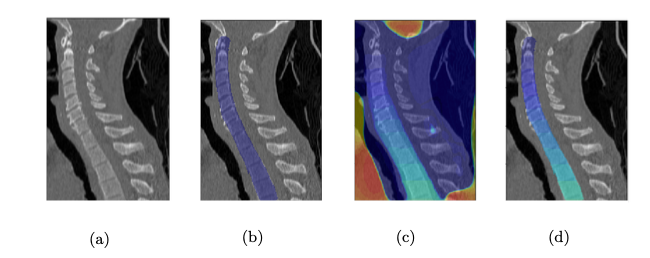
\includegraphics[width=9cm]{images/detection_identification_steps.png}
    \caption {(a) shows an original scan in grey-scale, (b) shows the output of the detection model applied to the scan, (c) shows the output of the identification model applied to the scan, (d) shows (b) and (c) multiplied together to produce a final prediction for each pixel.}
    \label{fig:detection_identification_steps}
\end{figure}


\section{Detection Model}

\section{Identification Model}